\documentclass[letterpaper]{article}
\usepackage[]{geometry}
\geometry{letterpaper}
\usepackage{graphicx}
\usepackage[utf8]{inputenc}
\usepackage{float}
\usepackage{fancyhdr}
\usepackage{multirow}
\bibliographystyle{IEEEtran}
\usepackage{enumitem}
\usepackage{amsmath}
\usepackage[hidelinks]{hyperref}
\usepackage{indentfirst}
\usepackage{comment}
\pagestyle{fancy}
\fancyhf{}
\lhead{UAFS Computer Science -- Capstone Proposal}
\rhead{Spring 2022}

\cfoot{\thepage}


%opening
\title{CombVCS - Combined Video Captioning and Search}
\author{An Le   \hspace{2em}   Jordan Aikey \hspace{2em} Julton Sword  \\[.5em]   Martin Tran  \hspace{2em}   Zachary Mackay \vspace{1em}}

\begin{document}
	
	
	
	%****************************************************************************************
	%  Title Page (minimum edits required)
	%****************************************************************************************
	
	
	\maketitle
	
	
	\begin{abstract}
		For this project, we propose CombVCS, a combined video captioning and search utility that will autonomously index a Smash Bros. Ultimate video and retrieve video clips utilizing a text-based search query. To accomplish this, the project employs methods from the fields of computer vision, natural language processing, and information retrieval. The project consists of a multi-step process: extract features from visual data, process features into text, index document features, and rank video timestamps based on relevancy to a search text query.
	\end{abstract}
	
	
	
	%****************************************************************************************
	%  Do not edit this section for any reason
	\begin{figure*}[!b]
		\centering
		
\includegraphics[width=0.25\linewidth]{uafsseal}\\[2em]
		\textsc{Department of Computer Science and Engineering} \\[0.5em]
		\textsc{University of Arkansas -- Fort Smith}
		\vspace{2em}
	\end{figure*}
	%**************************************************************************************** 
	
	\newpage
	
	%****************************************************************************************
	%  Table of Contents Page
	%****************************************************************************************
	
	\tableofcontents
	
	
	
	\newpage
	
	
	
	%****************************************************************************************
	%  Beginning of Content
	%****************************************************************************************
	
	
	
	
	
	
	%****************************************************************************************
	%  Introduction Section
	%****************************************************************************************
	
	\section{Introduction}
	
	Videos contain a large amount of data due to being composed of both visual and linguistic semantics. It can be an arduous task to locate portions of videos that contain relevant information. Advances in the field of natural language processing (NLP), computer vision, and machine translation have proven that machine learning models are capable of recognizing objects in images and describing the visual relationships in a natural language. Similar techniques for image-text tasks have been implemented into video-text tasks, in which the temporal visual semantics and their relationships in a video are described in a natural language. This project, CombVCS, is a video captioning and search utility that will autonomously index a Smash Bros. Ultimate video and implement a text-based video retrieval system. This project will borrow the works proposed by Luo\cite{luo2020univl}, Xu\cite{xu2016show}, and Merler\cite{merler2017automatic}. 
	
	\subsection{Problem Statement}
    When analyzing data contained in long videos, it is difficult and time-consuming to find points of interest where relevant events are occurring. Moreover, while analyzing videos, one must make an extensive catalog of each relevant event so that those events could be reexamined at a later date.  \\
	
	Classification of objects and events in video streams is an important concern for video data analysis tasks. One of the primary use cases for such systems is automated video surveillance analysis,  \cite{2021} but other areas of interest include computer vision for robotics, automated cars, and identification of useful information from recorded videos, such as determining where highlights have occurred in a sports game. \cite{merler2017automatic} Another use for automated video analysis is to help game developers grasp how players are utilizing various game mechanics by observing player streams on YouTube, Twitch, etc. This can help developers detect bugs and exploits more quickly after games are launched and updated. \\
	
	This project aims to solve the problem of streaming video processing and analysis using artificial intelligence (AI) and deep learning (DL) techniques. With sufficient data, AI and DL will automate this task and prevent situations in which human error could occur.
	
	
	
	\subsection{Objective}
	The goal for this project is to have a system automatically classify and index events of interest in a Super Smash Bros Ultimate game video stream.  The events of interest  are the moves that characters are executing and the interactions between characters that are competing. The system will create  timestamps that a user can access through a search engine to advance the video to specific times when those events of interest occurred. Finally, a user interface will link the analysis algorithm with the search engine, giving users a convenient way to seek events of interest in recorded video streams. \\
	
	Achievement of this objective is predicated on the completion of the following sub-goals:
	
	\begin{enumerate}
		\item \textbf{Construct dataset.} A custom dataset consisting of images captured from the Super Smash Bros. Ultimate video game is constructed. Images in the custom dataset are manually annotated with the target data which consists of the bounding region, identity, action, and effect of the characters on screen.
		
		\item \textbf{Identify characters and actions.} A neural network with object detection capabilities is implemented to determine the identity, location, and action of characters on the screen. A dataset comprised of annotated images is utilized to train and evaluate this model.
		
		\item \textbf{Identify the effect of a character's action.} A neural network with the capability to determine whether an attack resulted in the opposing character being hit, spiked, eliminated, or not affected. A dataset comprised of annotated images is utilized to train and evaluate this model.
		
		\item \textbf{Make data searchable.} Develop and utilize an information retrieval system that indexes the captions generated by the network and calculate each document score to determine relevancy against a search query. Users will have the ability to interact with the system through a web interface.
	\end{enumerate}
	
	%****************************************************************************************
	%  Background Section
	%****************************************************************************************
	
	\section{Background}
	
	The following sections will provide the necessary background and information regarding the technology to be utilized.
	
	\subsection{Overview}
	
	Artificial neural networks (ANN) are networks composed of neurons \cite{fnn}. Neurons are processing elements that lay at the foundation of a neural network. Neurons are able to accept input signals to process and send an output signal. Each neuron has at least one connection to another element in a network. This connection is called a weight coefficient and is represented by a real number. This weight reflects the degree of importance of the given connection. This number is computed using a weighted sum ($\sum_{i=0}^n x_iw_i$), where $x_i$ represents the input and $w_i$ represents the weight associated with that input at the $i^{th}$ location. Once the number is computed, it is sent into an activation function which acts as a gate to determine the output for the neuron. The image below visualizes one neuron \cite{perceptron1}.
	
	
	\begin{center}
		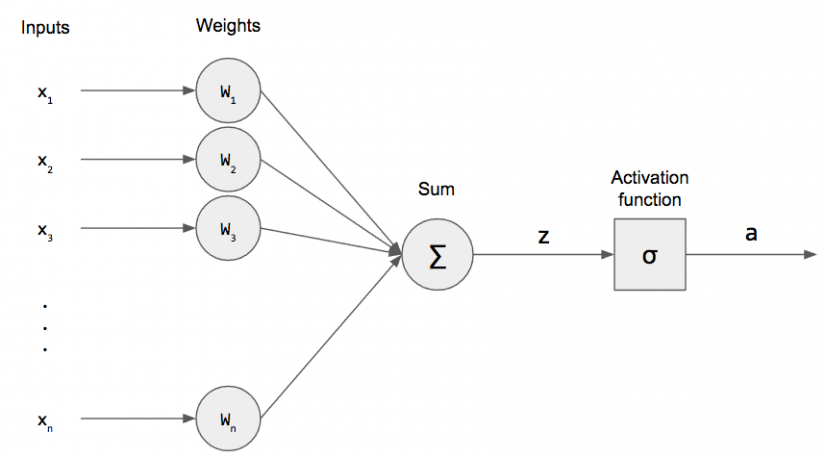
\includegraphics[scale=0.35]{perceptron}
	\end{center}
	
	
	A simple neural network model is a dense neural network. The term \emph{dense} describes all outputs of a given layer $i$ that has a connection to every input in layer $j$. Modern neural networks contain a combination of one or more layers that are composed of one or more neurons. This image shows the concept of a dense neural network \cite{perceptron2}.
	
	\begin{center}
		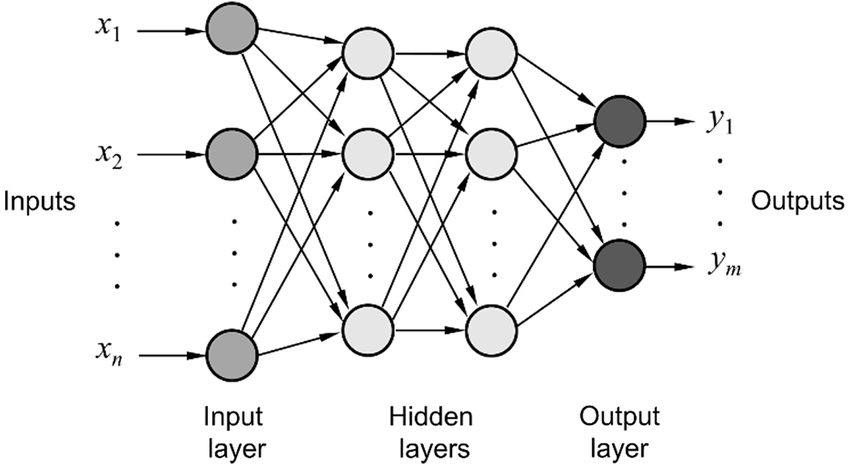
\includegraphics[scale=0.3]{multilayer_perceptron}
	\end{center}
	
	
	A convolutional neural network differs from a dense neural network in the following of ways. First, this network applies a filter by computing the dot product of the $m \times k$ input matrix and a $n \times n$ filter matrix. This dot product condenses the features from a region in the input matrix into smaller dimensions. This is repeated across the whole input, sliding the filter after each iteration until every feature is convolved. Filters are important in distinguishing points of interest from irrelevant information and reducing the dimensionality of the input \cite{featuremap}.
	
	\begin{center}
		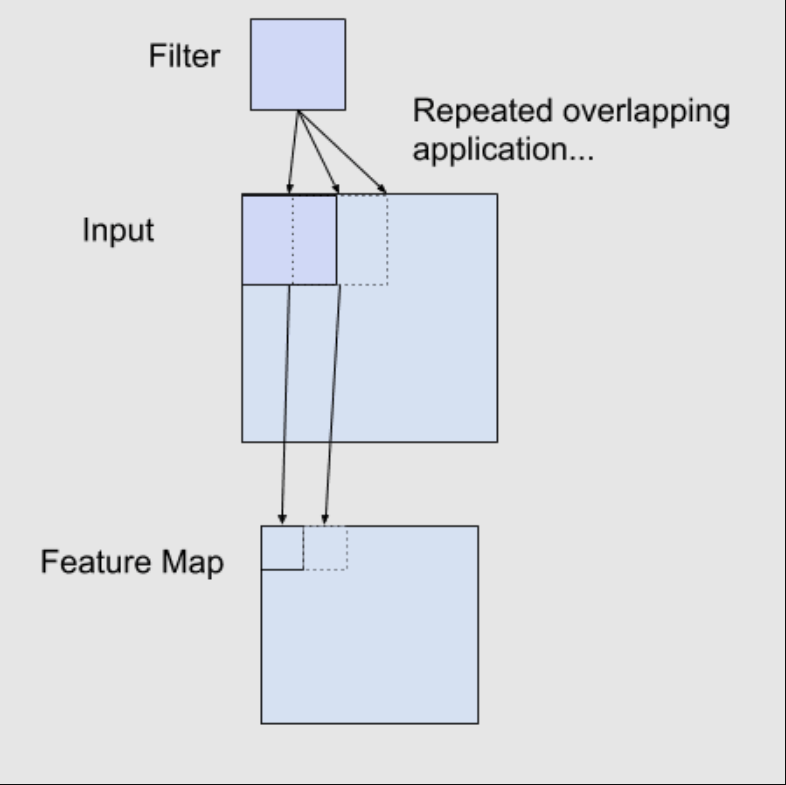
\includegraphics[scale=0.3]{feature_map}
	\end{center}
	
	\subsection{Technology}
	
	There exists a multitude of software applications, languages, and libraries that have been developed to aid code deployment in both research and production environments. The following are technologies that will be utilized for the project.
	
	\paragraph{Python}	Python is an interpreted high-level general-purpose programming language and emphasizes code readability. Python has gained high popularity in the field of machine learning and AI as Python has access to an extensive number of libraries that provide tools for machine learning and AI tasks. Python will serve as the primary programming language to develop and deploy this project's machine learning models and handle data transformation \cite{python1,python2}.
	
	\paragraph{Tensorflow}	Machine learning is an extensive field. Many tools have been developed to help implement and deploy AI models. Tensorflow, developed by the Google Brain team, is an end-to-end platform for machine learning. Tensorflow provides a high-level API for the development of machine learning models, deployment of distributed training, and usage of complex input data pipelines. Prominent users of Tensorflow include Intel, AMD, Nvidia, and Samsung Electronics. The primary task of Tensorflow for this project is to develop deep learning models through the Python programming language. \cite{tensorflow1,tensorflow2}.
	
	\paragraph{Vue.js}	Vue.js is an open-source front end JavaScript framework for building user interfaces and single-page applications. Prominent users of Vue.js include Google, Apple, and Nintendo. The primary task for Vue.js for this project is to aid development of a front end web page interface \cite{vue1,vue2}.
	
	\paragraph{Flask}	Flask is a micro web framework written in Python. It provides multiple tools and features for developing and deploying web applications in Python. Prominent users are Netflix, Reddit, Lyft, Airbnb, and MIT. Flask will provide a back-end environment to host this project's application.\cite{flask1,flask2}.
	
	
	\paragraph{OpenSUSE}	OpenSUSE is a community-developed Linux distribution developed by the openSUSE Project. OpenSUSE provides access to popular software and tools through the bundled package manager ZYpp and RPM. OpenSUSE also has built-in tools that allow for easy configuration of the system for task-specific use cases via command line or YaST. OpenSUSE is designed for desktop, workstation, and server environments. Prominent users of openSUSE or SLES include the Federal Emergency Management Agency, Lorven Technologies, and VMware Inc. OpenSUSE will serve as the primary operating system to host software or tools required by the project \cite{suse1,suse2}.
	
	
	
	
	\subsection{Related Work}
	
	\paragraph{Image Captioning}	Generating captions that describe an image is one of the primary goals of computer vision. This task requires both natural language processing and computer vision techniques. Not only must caption generation models be powerful enough to determine which objects are in an image, but they must also be capable of capturing and expressing their relationships in a natural language. Multi-modal attention networks have improved the quality of image-text tasks through the use of large scale datasets, convolutional neural networks, and recurrent neural networks combined with attention mechanisms \cite{xu2016show}.
	
	\paragraph{Video Captioning}Today, there is an extraordinary amount of visual data which has bred an increasing interest in advancing video understanding \cite{princeton}. The video captioning problem arises as the next natural step where a sentence or paragraph is generated to describe a video's visual semantics. Video captioning is similar in nature to image captioning, but differs due to a temporal factor. This presents a new set of challenges for a model such as describing a combination of arbitrary sequential frames, and text-based video retrieval. UniVL achieved state-of-the-art results through the usage of multimodal networks and large scale datasets. UniVL consists of four components, including two single modal encoders, a cross encoder, and a decoder with the Transformer backbone \cite{luo2020univl}.
	
	\paragraph{Excitement Features}	Novel techniques to generate natural language text for video have achieved state-of-the-art results. These approaches have leaned heavily on deep learning to determine the relationships between the visual and text semantics. The works proposed by Merler \cite{merler2017automatic} utilized excitement features of visual, text, and audio as markers to relevant highlights of a video. By utilizing these markers, this eases the task for models to determine the high-profile events that occur within a video. Multiple models are utilized to extract features regarding their domain, determine excitement indicators, and extract relevant frames of a video.
	
	%****************************************************************************************
	%  Design Section
	%****************************************************************************************
	
	
	\section{Design}
	
	The design of this project will have the following requirements:
	\begin{itemize}
		\item A system of image recognition networks that can identify characters, actions, and events inside of the Super Smash Bros. Ultimate video game.
		\item A document indexing/retrieval system to serve as a search engine to query the captions belonging to a video clip, retrieve time stamps of the closest result, and display the time stamps to the user.
	\end{itemize}
	
	\subsection{Project Requirements}
	
	\begin{enumerate}
		\item{
			GPU (accelerator) - increases performance significantly
		}
		
		\item{
			Gitea - collaboration and version control
		}
		
		\item{
			Nintendo Switch - platform to run the video game
		}	
		
		\item{
			Super Smash Bros. Ultimate - media that the project is based on
		}
		
		\item{
			El Gato - enables screen capturing from the Nintendo Switch gaming console
		}
		
		\item{
			Television - output for the Nintendo Switch
		}
		
		\item{
			Linux Computer - utilized to run the project and access the feed given from the El Gato 
		}
		\item{
			Google Colaboratory  -  allows for a cloud-based usage of a GPU
		}
	\end{enumerate}
	
	
	\subsection{Architecture}
	
	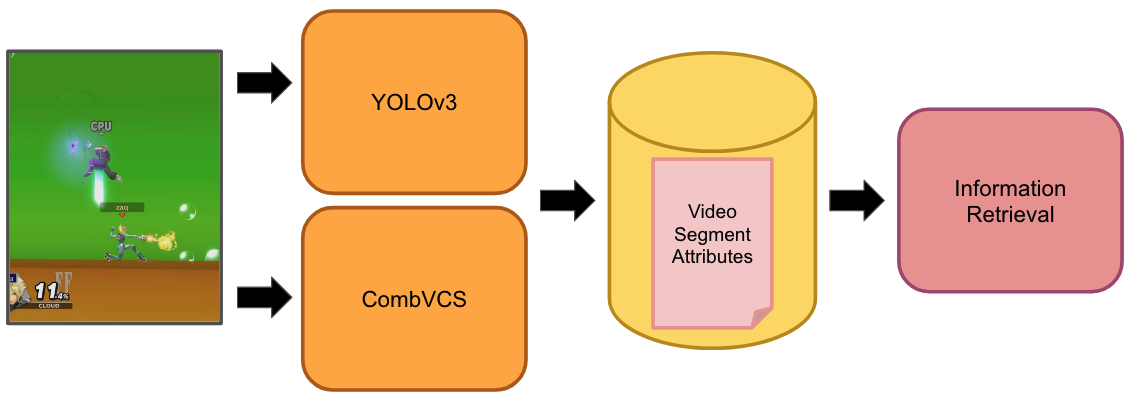
\includegraphics[width=.93\linewidth]{system.png}
	
	\paragraph{YOLOv3} For character detection and boxing, this project utilizes the same architecture outlined in YOLOv3\cite{yolov3}, which is a highly effective object detection model in both speed and performance. This model consists of several skip connections, convolutional layers, and max pooling layers to encode images. Up-sampling layers are utilized to increase the scale of the encoded image which improves the ability of deeper classification heads to detect the presence of small objects.
	\begin{center}
		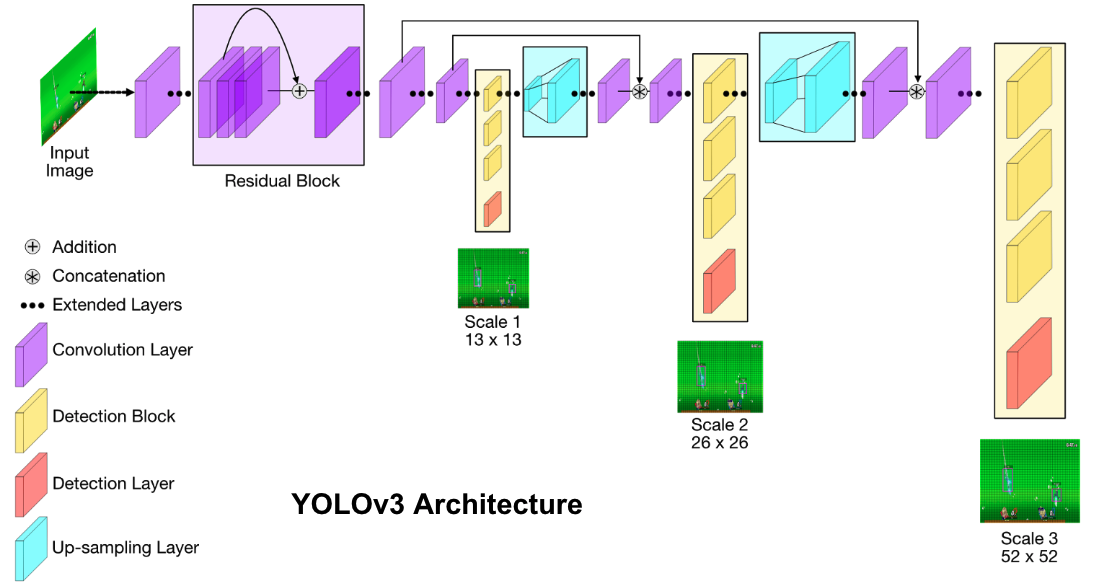
\includegraphics[width=.9\linewidth]{yolov3.png}
	\end{center}
	
	\paragraph{Effects Model} A convolutional neural network is leveraged to identify effects that occurred. This model consists of several convolutional and max pooling layers to encode the image. The encoded image is classified using dense neural layers to determine the presence of an effect. This model utilizes the Adam optimizer, a learning rate of $0.001$, ReLU and softmax activation functions and a categorical cross entropy loss.\\
	\begin{center}
	   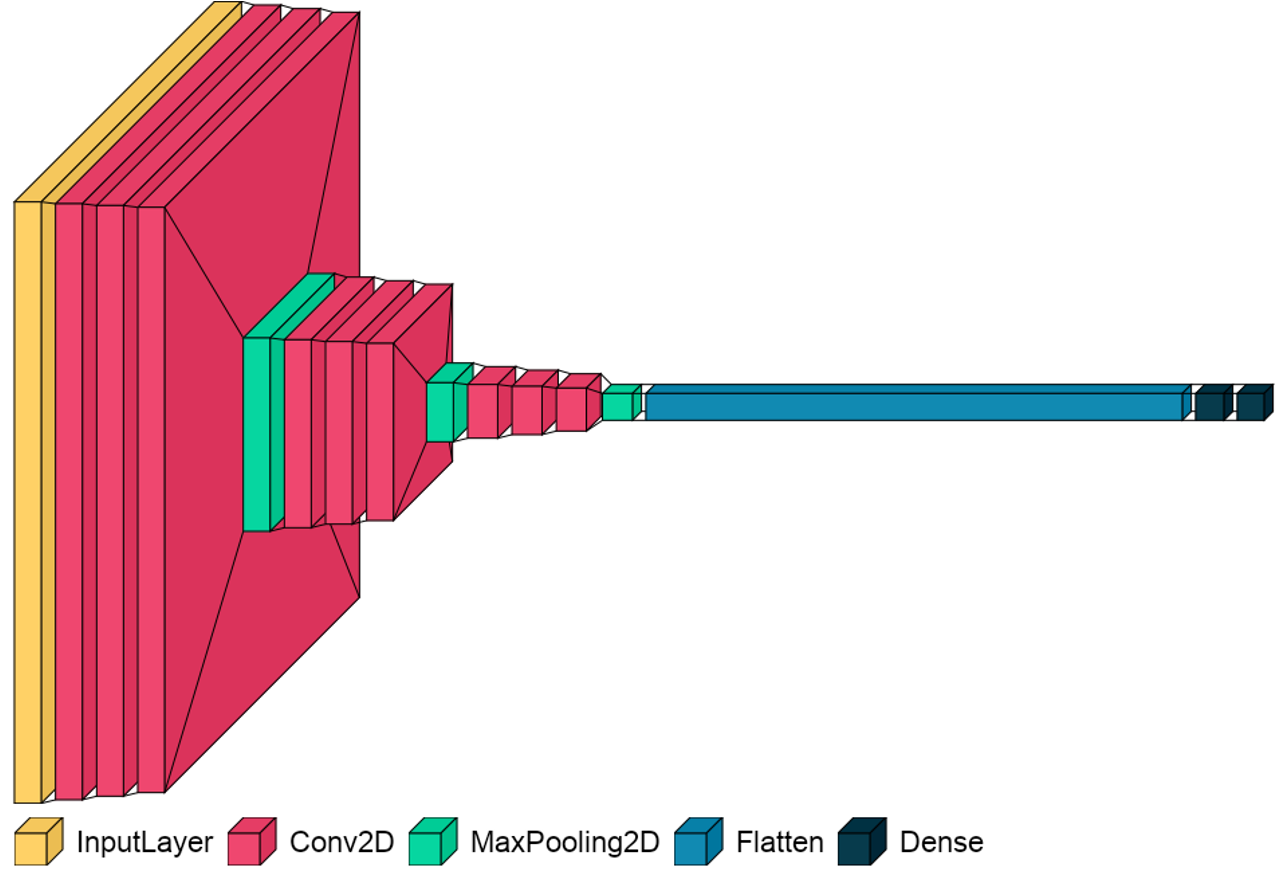
\includegraphics[width=.60\linewidth]{effects_model.png} 
	\end{center}
	
	\paragraph{Information Retrieval} For the information retrieval portion of the system, a TF-IDF vectorizer is utilized to project each document into a vector space. By using the TF-IDF vectors along with pairwise cosine similarity, the information retrieval system provides the ability to search for events within a video that has been processed by the cognitive analysis components of the system to retrieve relevant timestamps.
	
	
	\subsection{Risks}
	

		\paragraph{Overfitting}	Various techniques will be employed as needed to reduce overfitting, including adjusting the size and variety of training data, controlling the number of training epochs for neural networks, and randomly altering image features. 
		
		\paragraph{Insufficient Training Data} Although video streams of Smash Bros. Ultimate games are widely available, this project requires a specialized set of training videos and images to train the neural networks that are responsible for event classification and indexing. This task will require a significant amount of time and must be managed carefully.
		
		\paragraph{Excessive Training Time}	Due to the large number of characters, move sets, and variations in appearance in Smash Bros. Ultimate, it is necessary to process numerous images and video clips to train the neural networks that are responsible for event classification and indexing. Thus, efficient algorithms and data storage techniques are necessary to ensure computational complexity and neural network training times do not become impossibly large.
		
		\paragraph{User Input Errors}	While the need for user input for this application is minimal (primarily restricted to use of the search engine), some simple input sanitization and validation techniques are employed to avoid potential bugs and unexpected behavior.
	
	
	\subsection{Tasks}
	
	\begin{enumerate}
		\item{
			Research and gain understanding of the approach that will be taken.
		}
		
		\item{
			Gather and label data. The training data will consist of labeled images of Smash Bros. characters executing different actions within the video game. 
		}
		
		\item{
			Design and build machine learning models. This will consist of pre-trained image recognition models that are fine tuned for this projects tasks.
		}
		
		\item{
			Design and build a document indexing system.
		}
		
		\item{
			Design and build an information retrieval system that will execute a text search query and retrieve relevant video clips. 
		}
		
		\item{
			 Evaluate, optimize, and update the models.
		}
		
		\item{
			Report performance and final model architecture, as well as any other findings. 
		}
	\end{enumerate}
	
	\section{Experimentation}
	
	\subsection{Character Detection}
	
	A baseline custom network was constructed for performance comparison. Initial network experiments followed VGG-16 \cite{vgg16} and ResNet50 \cite{resnet50} architectures. Each network was trained and evaluated on the same data split. Although each network displayed the ability to bound and classify characters, after visual evaluation of the testing data split, each model consistently predicted bounding boxes that were incorrectly positioned. YOLOv3 delivered promising results compared to the previous architectures. YOLOv3 takes in consideration a 'confidence level' to determine the presence of an object within a bounded region. Compared to the initial networks that utilize a mean-squared-error loss, YOLOv3 leverages intersect-over-union loss for boxing, which we hypothesize stabilized training.
	
	\subsection{Effect Detection}
	
	A convolutional neural network was constructed to classify the presence of an elimination or spike occurring in the frame. This network consisted of several convolutional layers followed by max pooling layers. The encoded image would then be passed into a dense neural head to classify the presence of a target event. Adjustments in the network's architecture included the frequency of layers and the number of neurons per layer. These adjustments did not have significant impact on performance.

	\newpage
	
	\section{Results}
	
	The effects model trained across 50 epochs with 80\% of the data reserved for training and 20\% for testing respectively. The YOLOv3 model was trained across 236k epochs with an early stopping delta loss criteria. The model converged at 47k epochs. Human evaluation of the information retrieval system was conducted to determine the performance and relevancy of the retrieved timestamps.
	  
	\begin{figure}[H]
		\centering
		\begin{minipage}{.48\linewidth}
			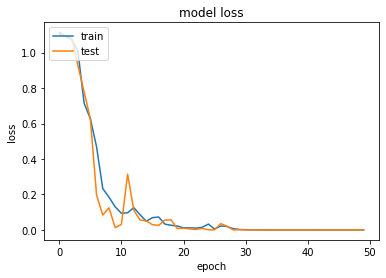
\includegraphics[width=\linewidth]{loss_effects.png}
			\caption{Effects model loss}
			\label{img1}
		\end{minipage}
		\hfill
		\begin{minipage}{.48\linewidth}
			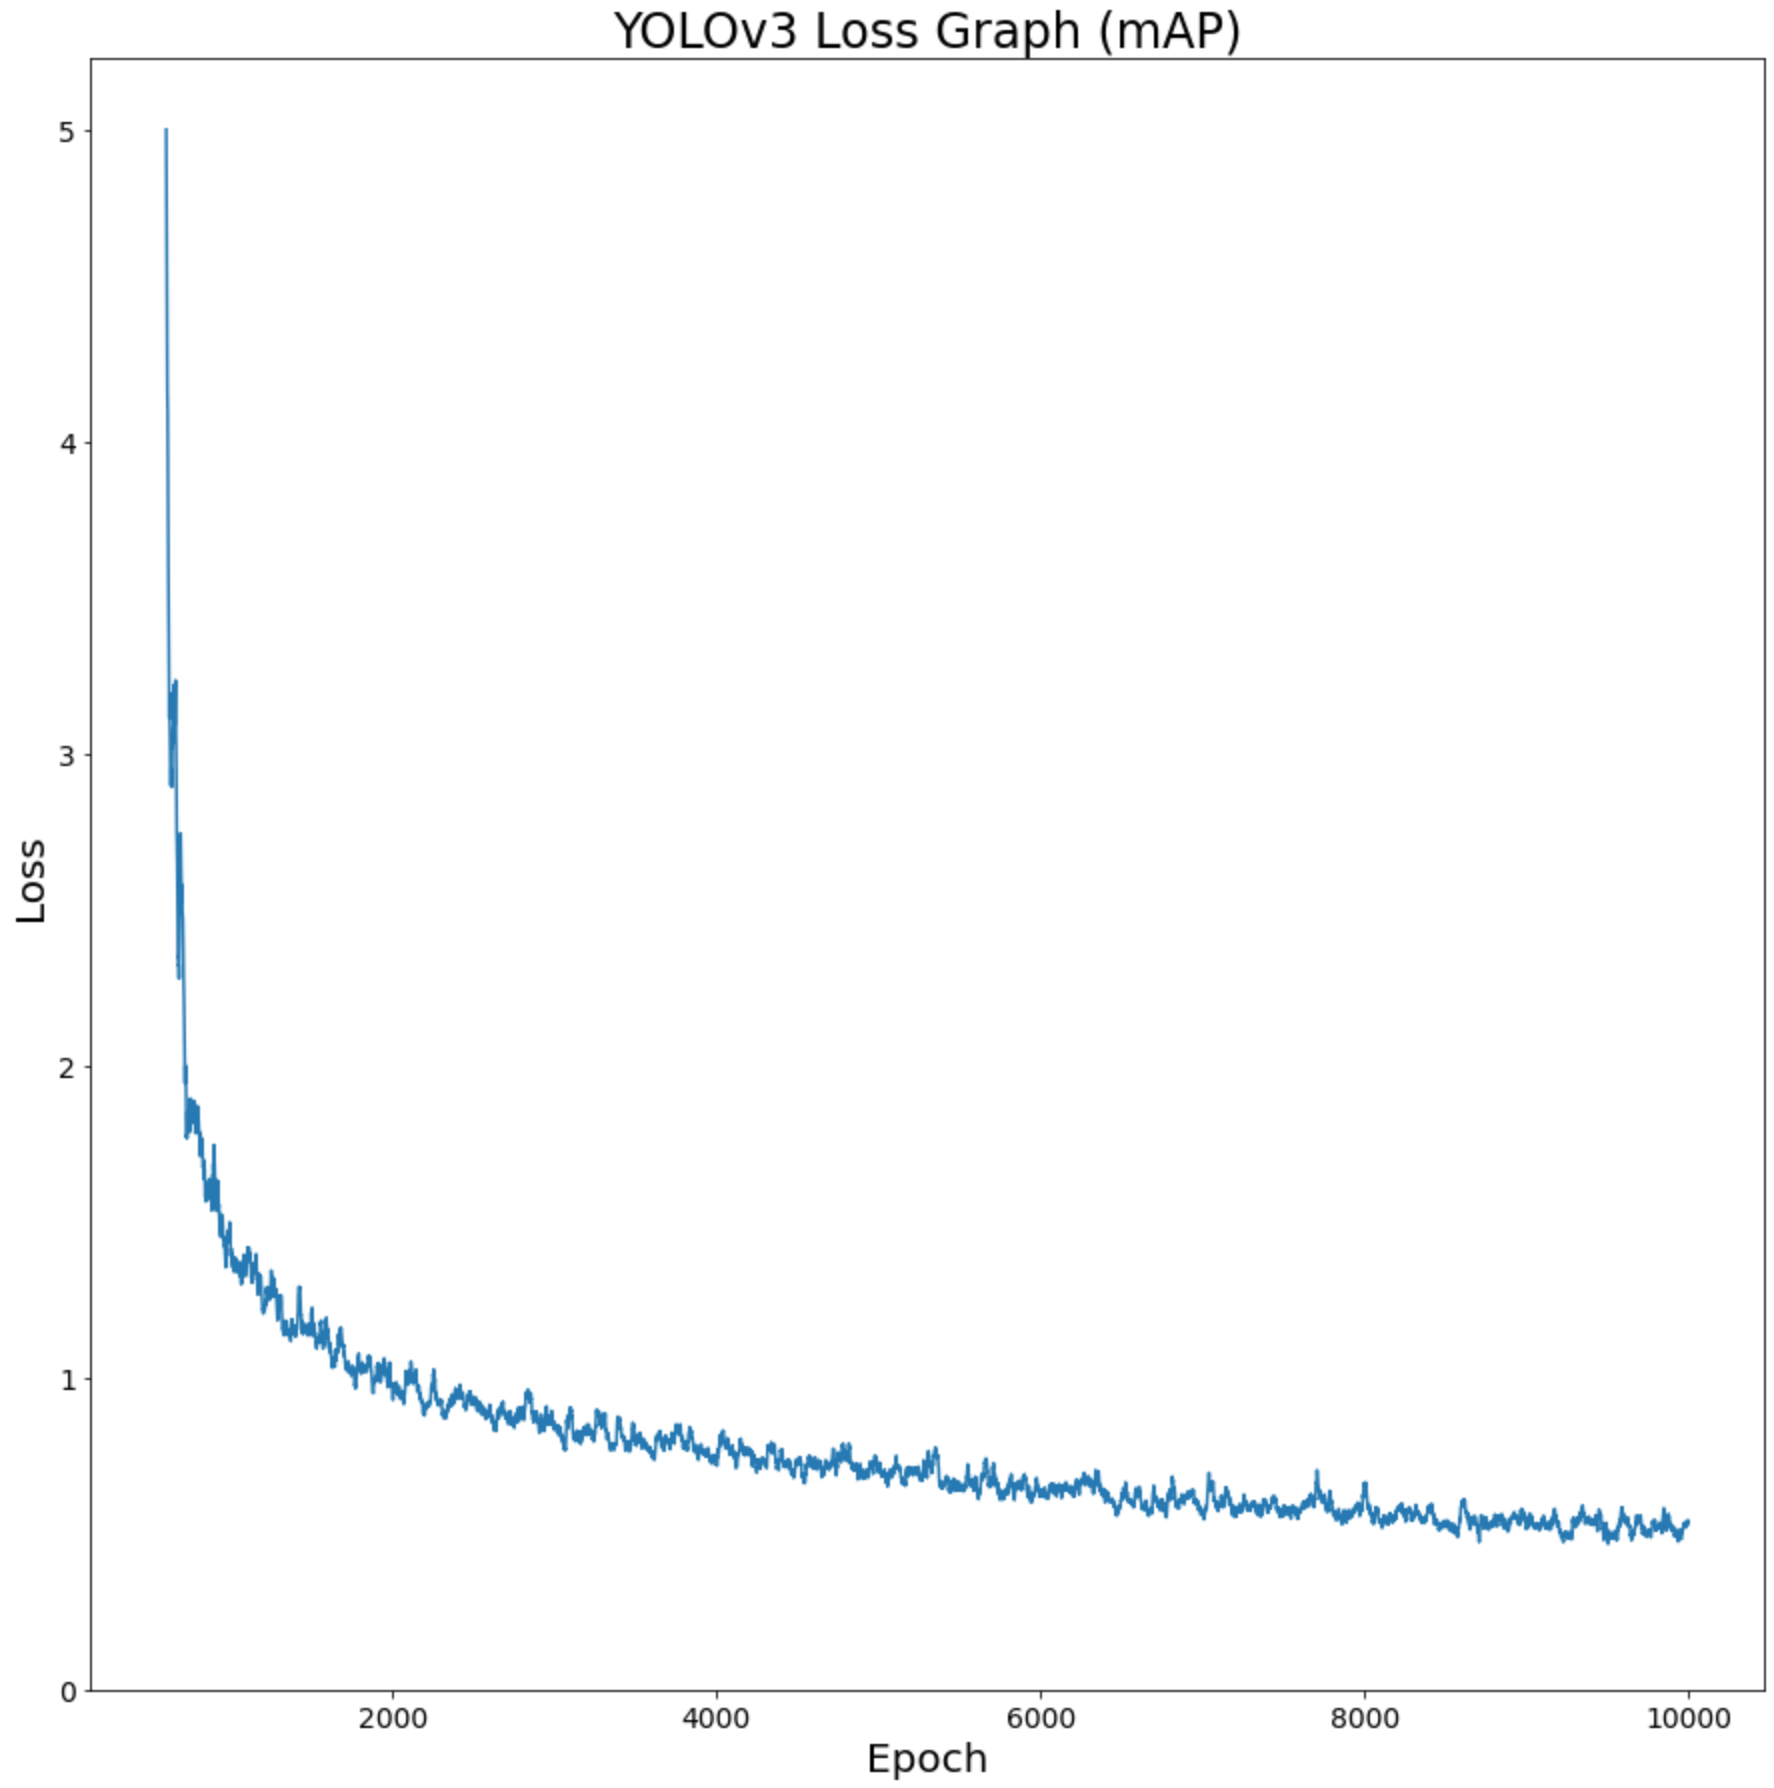
\includegraphics[width=\linewidth]{loss_yolov3.png}
			\caption{YOLOv3 model loss}
			\label{img2}
		\end{minipage}
	\end{figure}
	
	\subsection{Screenshots}
	\noindent
	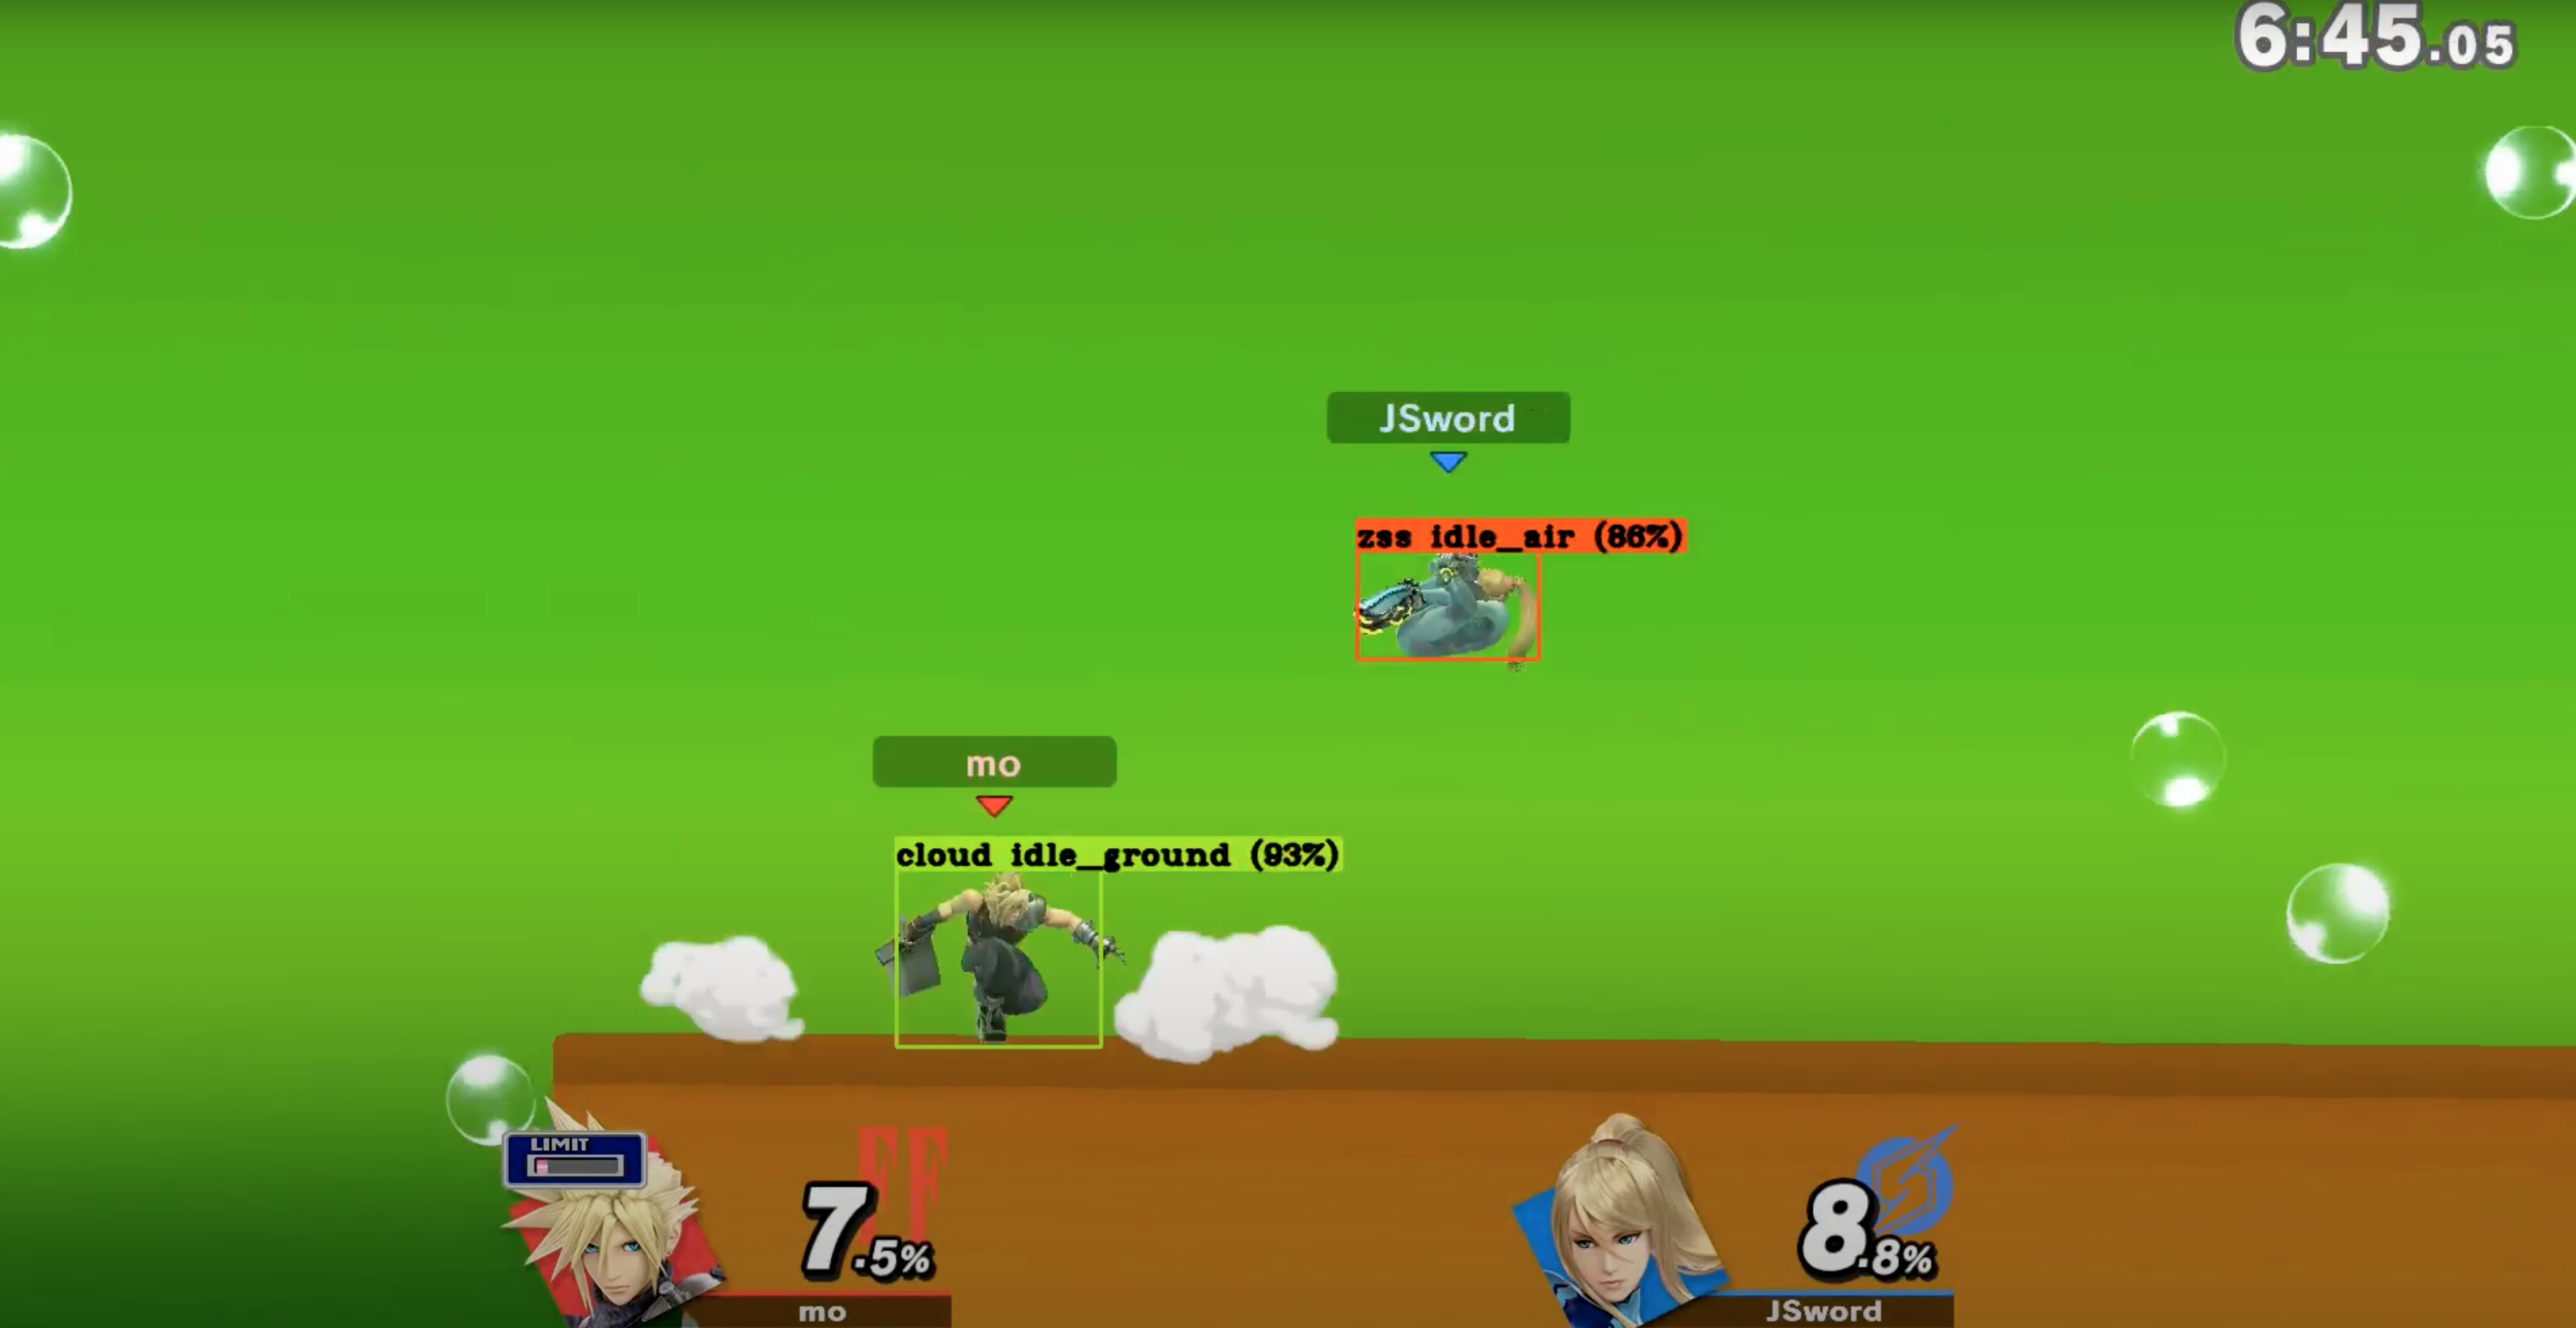
\includegraphics[width=\textwidth]{yolo_in_effect.png}
	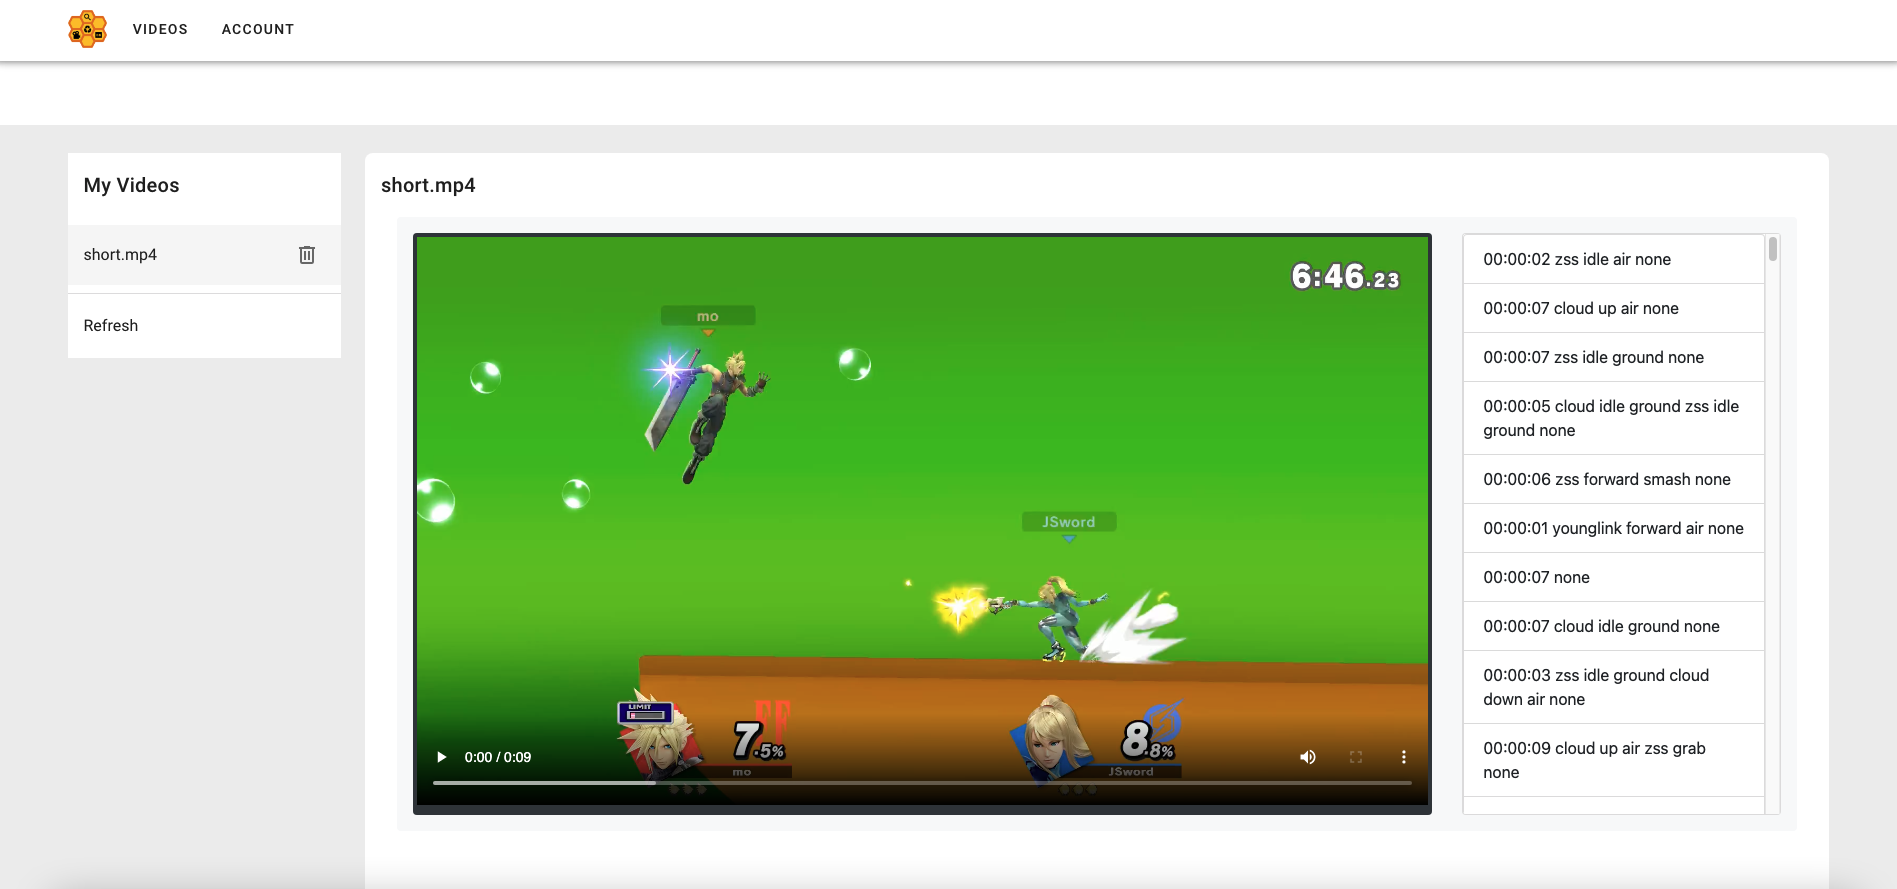
\includegraphics[width=\textwidth]{website2.png}
	
	
	\subsection{Schedule}
	
	\begin{center}
		\resizebox{\columnwidth}{!}{%
			\begin{tabular}{ |p{3cm}|p{3.2cm}|p{3cm}|p{3cm}|p{3cm}|  }
				\hline
				\multicolumn{5}{|c|}{Schedule} \\
				\hline
				Sprint 1 & Sprint 2  & Sprint 3 & Sprint 4 & Final\\
				\hline
				\hline
				Research &   Build character identification network  &  Design network to identify a character’s move effect (spike, none, elim.)&  Design autonomous captioning and indexing system &   Showcase project \\
				\hline
				Gather and label data   &  Train and tune character identification network   & Label the rest of the data  & Build autonomous captioning and indexing system. & Report findings  \\
				\hline
				Design model to identify character   &  Build character action identification network    & Combine character action and identification using YOLOv3 & Implement search engine  & Poster \\
				\hline
				Design model to identify character's action &  Train and tune character action network   &  Train the YOLOv3 classification system & Design a search engine to allow the retrieval of indexed events & Design logo  \\
				\hline
				&  Gather and label more data & & &   \\
				
				\hline
		\end{tabular}}
	\end{center}
	
	\subsection{Deliverables}
	
	\begin{enumerate}
		\item Project Proposal and Presentation
		\item User Interface Design and Application
		\item Machine Learning Model Code 
		\item Application Development Code 
		\item Project Poster
		\item Final Report
	\end{enumerate}

	%****************************************************************************************
	%  Members Section
	%****************************************************************************************
	
	
	
	\section{Project Members}
	
	In this section, all project members and advisors are presented.
	
	\subsection{Team Members}
	
	\paragraph{Zachary Mackay(Data Science/Artificial Intelligence)} Zachary Mackay is Computer Science major with concentration in Data Science and Artificial Intelligence and a minor in Mathematics in the department of Computer Science and Engineering at the University of Arkansas -- Fort Smith. He has completed relevant coursework for the proposed project by completing CS 3113 -- Artificial Intelligence, CS 4143 -- Deep Learning, CS 4333 -- Machine Learning. His responsibilities will include data collection and labeling, designing and implementing the model, researching similar projects to aid in producing the best possible outcome. \\
	
	\paragraph{Martin Tran (Data Science/Artificial Intelligence)} Martin Tran is a Computer Science major in the department of Computer Science and Engineering at the University of Arkansas - Fort Smith. He has completed relevant coursework for the proposed project by completing CS 3113 -- Artificial Intelligence, CS 4343 -- Natural Language Processing, CS 4903 -- Deep Learning, and CS 4333 - Machine Learning. He also obtained research experience as a member of the UAFS Artificial Intelligence Research Lab. His responsibilities will include the data collection, data processing, model optimization, and development of a web application. \\
	
	\paragraph{Julton Sword (Data Science/Artificial Intelligence)} Julton Sword is a Computer Science major in the department of Computer Science and Engineering at the University of Arkansas - Fort Smith. He has completed relevant coursework for the proposed project by completing CS 3113 -- Artificial Intelligence, CS 4343 -- Natural Language Processing,  and CS 4333 -- Machine Learning, and he is currently taking CS 4143 -- Deep Learning. His responsibilities will include preparing logic to process training data, setting up neural network model architecture, researching technologies and techniques to improve model performance, and designing user interface components. \\
	
	\paragraph{Jordan Aikey (Data Science/Artificial Intelligence)} Jordan Aikey is a Computer Science major with a concentration in Data Science and Artificial Intelligence and a minor in Mathematics in the department of Computer Science and Engineering at the University of Arkansas -- Fort Smith. He has completed relevant coursework for the proposed project by completing CS 3113 -- Artificial Intelligence, CS 4333 -- Machine Learning, and CS 4373 -- Information Retrieval. Additionally, he is currently taking CS 4143 -- Deep Learning. He is currently obtaining relevant research experience as a Lab Assistant in the UAFS Artificial Intelligence Research Lab. His responsibilities will include data collection, research and development of image recognition models, research and development of NLP/NLG models, and research and development of a search engine. \\
	
	\paragraph{An Le (Data Science/Artificial Intelligence)}  An Le is a Computer Science major and a minor in Mathematics in the department of Computer Science and Engineering at the University of Arkansas -- Fort Smith.  He has completed relevant coursework for the proposed project by completing CS 3113 -- Artificial Intelligence, CS 4343 -- Natural Language Processing, CS 3323 -- Computer Graphics, and CS 4333 -- Machine Learning. In addition, he obtained research experience as a member of the UAFS Artificial Intelligence Research Lab. His responsibilities will include processing training data, development of machine learning models, and backend development of this project’s text-based video retrieval system. \\
	
	\subsection{Departmental Advisors}
	
	\paragraph{Andrew Mackey}Our project was supervised by Professor Andrew Mackey in the department of Computer Science and Engineering at the University of Arkansas -- Fort Smith. He oversees the UAFS programming team as well as the UAFS Artificial Intelligence Research Lab. He has published multiple papers in the field of information systems, machine learning, natural language processing, and computer vision.
	
	\paragraph{Israel Cuevas}Our project was supervised by Professor Israel Cuevas in the department of Computer Science and Engineering at the University of Arkansas -- Fort Smith. He has published multiple papers in the field of machine learning, natural language processing, and computer vision.
	
	
	%****************************************************************************************
	%  References Section
	%****************************************************************************************
	\bibliography{refs}
	
\end{document}
